% Copyright 2010 by Frank Wood

\documentclass{beamer}
\usepackage{algorithm}
\usepackage{algorithmic}
\usepackage{natbib}

% Setup appearance:

\usetheme{Darmstadt}
\usefonttheme[onlylarge]{structurebold}
\setbeamerfont*{frametitle}{size=\normalsize,series=\bfseries}
\setbeamertemplate{navigation symbols}{}

% Standard packages

\usepackage[english]{babel}
%\usepackage[latin1]{inputenc}
%\usepackage{times}
%\usepackage[T1]{fontenc}
%\usepackage{nnfootnote}
\usepackage{amsfonts}
\usepackage{amsmath}

% Setup TikZ

%\usepackage{tikz}
%\usetikzlibrary{arrows}
%\tikzstyle{block}=[draw opacity=0.7,line width=1.4cm]


% Author, Title, etc.

\title[Applied Nonparametric Bayesian Modeling] 
{
  Applied Nonparametric Bayesian Modeling
}

\author[Wood]
{
  Frank~Wood%\inst{1}
}

\institute[Columbia University]
{
  %\inst{1}%
  Columbia University
}

\date[Job Talk 2010]
{Job Talk 2010}

%\def\blfootnote{\xdef\@thefnmark{}\@footnotetext}


% The main document

\begin{document}
\newcommand{\ubf}{\mathbf{u}}
\newcommand{\xbf}{\mathbf{x}}
\newcommand{\sbf}{\mathbf{s}}
\newcommand{\py}{\mathcal{PY}}
\newcommand{\vbf}{\mathbf{v}}
\newcommand{\Prob}{\mathrm{P}}
\newcommand{\Psmooth}{\Prob_\text{smooth}}
\newcommand{\parent}{\pi}
\newcommand{\suffix}{\sigma}
\newcommand{\UHPYP}{SM}
\newcommand{\PLUMP}{PLUMP}
\newcommand{\Oh}{\mathcal{O}}
\newcommand{\tree}{\mathcal{T}}

% \newcommand{\cusk}{c_{\ubf s k}}
% \newcommand{\cus}{c_{\ubf s \cdot}}
% \newcommand{\cu}{c_{\ubf \cdot \cdot}}
% \newcommand{\tus}{t_{\ubf s}}
% \newcommand{\tu}{t_{\ubf \cdot}}
\newcommand{\cusk}{c_{\ubf s k}}
\newcommand{\cus}{c_{\ubf s}}
\newcommand{\cu}{c_{\ubf \cdot}}
\newcommand{\tus}{t_{\ubf s}}
\newcommand{\tu}{t_{\ubf \cdot}}
\newcommand{\cset}{\{\cusk\}_{s\in \Sigma,k \in \{1,\ldots,t_{\ubf s}\}}}
\newcommand{\tset}{\{\tus\}_{s\in \Sigma}}
\newcommand{\bydef}{\equiv}
\newcommand{\state}{\mathcal{S}_{\xbf}}
\newcommand{\statei}{\mathcal{S}_{\xbf_{1:i}}}
\newcommand{\emptystring}{\varepsilon}
\newcommand{\gcount}{\hat{c}}
\newcommand{\escape}{\mathtt{esc}}

\newcommand{\todo}[1]{\begin{center}\textbf{TODO: } #1 \end{center}}
\newcommand{\figref}[1]{\figurename~\ref{#1}}
\newcommand{\predictive}{\Prob(x_i|\xbf_{1:i-1})}
\newcommand{\ywcomment}[1]{\textbf{#1}}
\newcommand{\jgcomment}[1]{ { \textcolor{red}{#1} } }



%\nofootnotemark
\begin{frame}
  \titlepage
\end{frame}

\begin{frame}{Outline}
  \tableofcontents
\end{frame}

\section{Motivation}
\subsection{Example}
\section{Background}
% !TEX root = talk.tex
\begin{frame}[t]{Definition}
\begin{block}{Dirichlet Process (DP), \citet{Ferguson1973}}
We say
 \[G \sim \DP(c,G_0)\]
 if for any partition $A_1, \ldots, A_k$ of the sample space, the vector of random probabilities
$[G(A_1), \ldots, G(A_k)]$ follows a Dirichlet distribution, i.e.
\[[G(A_1), \ldots, G(A_k)] \sim \Dir(cG_0(A_1), \ldots, cG_0(A_k))\]
\end{block}
\end{frame}	

\begin{frame}[t]{Properties}
\begin{block}{Basics}
\begin{eqnarray*} 
[G(A),G(A^C)] \sim \Dir(cG_0(A), cG_0(A^C)) 
\end{eqnarray*}
reduces to
\[G(A) \sim \Bet(cG_0(A), cG_0(A^C))\]
which means
\[ \Ave(G(A)) \comment{= \frac{cG_0(A)}{cG_0(A)+cG_0(A^C)}} = G_0(A)\] 
and
 \begin{eqnarray*} 
\Var(G(A)) &=& \comment{\frac{c^2G_0(A)G_0(A^C)}{(cG_0(A)+cG_0(A^C))^2(cG_0(A)+cG_0(A^C)+1)} \\
&=&} \frac{G_0(A)(1-G_0(A))}{(c+1)}
 \end{eqnarray*}
\end{block}
 Note, as $c\rightarrow\infty, \Var(G(A))\rightarrow0$ and thus $G(A) \rightarrow G_0(A)$
\end{frame}	

\begin{frame}[t]{Explicit Construction}
\begin{block}{\citet{Sethuraman1994a}}
\[G(\cdot) = \sum_{k=1}^\infty w_k \delta_{\phi_k}(\cdot)\]
where 
\[{\phi_k} \sim G_0 \mbox{ and } w_k = V_k\prod_{j<k}(1-V_j), V_k \sim \Bet(1,c)\]
\end{block}
Note: this is known as the ``stick-breaking'' construction.
\end{frame}	

\begin{frame}[t]{Efficient Posterior Updating}
\begin{block}{Polya Urn \citep{Blackwell1973}}
\begin{eqnarray*}
x_1 &\sim& G_0 \\
G | x_1 &\sim& \DP\left(1+c, \frac{1}{1+c}\delta_{x_i} + \frac{c}{1+c}G_0\right)\\
x_2 | x_1 &\sim& \frac{1}{1+c}\delta_{x_i} + \frac{c}{1+c}G_0 \\
G | x_1, x_2 &\sim& \DP\left(2+c, \frac{1}{2+c}\sum_{i=1}^n \delta_{x_i} + \frac{c}{2+c}G_0\right)\\
&\vdots&\\
\end{eqnarray*}
\end{block}
\end{frame}	


\begin{frame}[t]{Efficient Posterior Updating}
\begin{block}{Polya Urn \citep{Blackwell1973} Cont.}
\begin{eqnarray*}
x_n | x_1,\ldots x_{n-1} &\sim& \frac{1}{n-1+c}\sum_{i=1}^{n-1}\delta_{x_i} + \frac{c}{n-1+c}G_0 \\
G | x_1, \ldots, x_n &\sim& \DP\left(n+c, \frac{1}{n+c}\sum_{i=1}^n \delta_{x_i} + \frac{c}{n+c}G_0\right)
\end{eqnarray*}
Note: 
\begin{itemize}
\item Neither posterior predictive nor posterior distributions depend on the order of the $x_i$'s ($x_i$'s ``exchangeable'')
\item Many $x_i$'s will share the same value, call a shared value $\phi_k$
\item ``Observing'' $\phi_k$ once increases probability of observing it again and this is reinforced
\end{itemize}
\end{block}
\end{frame}	

\begin{frame}[t]{Incremental Estimation}
\begin{block}{Sequential Monte Carlo}
The posterior distribution is fully characterized by 
\[\frac{1}{n-1+c}\sum_{i=1}^{n-1}\delta_{x_i} + \frac{c}{n-1+c}G_0\]
Particle filters for posterior estimation in general DP models can be constructed by, for each new observation either
\begin{itemize}
\item {\em Sampling}
\item {\em Enumerating} 
\end{itemize}
whether the observation arose from
\[\frac{1}{n-1+c}\sum_{i=1}^{n-1}\delta_{x_i}  \quad \mbox{      or        } \quad \frac{c}{n-1+c}G_0\]
\end{block}
\end{frame}

\begin{frame}[t]{Incremental Estimation}
\begin{block}{Sequential Monte Carlo}
In the discrete likelihood case, an ``efficient''  {\em single}-particle particle filter posterior estimator consists of a particle $\ell = 1$ containing a set of draws from the base distribution 
\[\Phi_\ell = \{\phi_k\}_{k=1}^K, \phi_k \sim G_0\]
and a set of counts, one per $\phi_k$, indicating how many times each draw from the base distribution was responsible for generating an observation
\[{\bf c}_\ell = \{c_k\}_{k=1}^K\]
\end{block}
Note, $K\leq N$
\end{frame}

\begin{frame}[t]{Uses}
\begin{block}{Density Estimation, Mixing A Smooth Kernel}
Dirchlet Process Mixture model \citep{Escobar1995, MacEachern1998, Neal1998}
\begin{eqnarray*}
G &\sim& \DP(c,G_0) \\
\theta_i &\sim& G \\
x_i | \theta_i &\sim& F(\theta_i),
\end{eqnarray*} 
or equivalently%
\begin{eqnarray*}
z_i &\sim& \CRP(c) \\
\theta_k &\sim& G_0 \\
x_i | z_i &\sim& F(\theta_{z_i})
\end{eqnarray*} 

\end{block}

Note: constructing SMC or MCMC samplers for either of these representations is more complicated but still straightforward.
\end{frame}	


\begin{frame}[t]{Uses}
\begin{block}{Hierarchical Dirichlet Process \cite{Teh2006b}}
Dirichlet processes can be used as ``glue'' to hierarchically tie together distributions governing related populations in order to ``share statistical strength'' during inference.
\begin{columns}[t]
\begin{column}{.5\textwidth}
\begin{eqnarray*}
G &\sim& \DP(c,G_0) \\
G_j &\sim& \DP(c,G) \\
\theta_{ij} &\sim& G_j \\
x_{ij} | \theta_{ij} &\sim& F(\theta_{ij}),
\end{eqnarray*} 
\centering
\hspace{.25cm} here $G_j$ is a per-class distribution over population {\em parameters}.
\vspace{2cm}
\end{column}
\begin{column}{.5\textwidth}
\begin{figure}
\begin{center}
\includegraphics[trim = 4cm 8cm 4cm 8cm, clip, width=5cm]{fig/shared_clustering.pdf}
%\caption{Shared clustering}
\label{default}
\end{center}
\end{figure}
\end{column}
\end{columns}
\end{block}
\end{frame}	


\begin{frame}[t]{Hierarchical Dirichlet Process Inference}
%SMC and MCMC algorithms based on the Polya urn representation exist for hierarchical DP's as well.  
Consider the ``full characterization'' of the posterior predictive distribution of the base level of a DP model
\begin{eqnarray*}
G &\sim& \DP(c,G_0) \\
G_j &\sim& \DP(c,G) \\
\theta_{ij} &\sim& G_j \\
\end{eqnarray*} 
i.e.
\[\theta_{nj} | \theta_{1j}, \ldots, \theta_{n-1,j} =  \frac{1}{n-1+c}\sum_{i=1}^{n-1}\delta_{\theta_{ij}} + \frac{c}{n-1+c}G_j\]

\end{frame}

\begin{frame}[t]{Hierarchical Dirichlet Process Inference}
Now consider $G_j$ as having been similarly marginalized out and represented in the same way

\[\psi_{nj} | \psi_{1j}, \ldots, \psi_{n-1,j} =  \frac{1}{n-1+c}\sum_{i=1}^{n-1}\delta_{\psi_{ij}} + \frac{c}{n-1+c}G\]
Consider the following argument.  If $\theta_{nj} \notin \{\theta_{ij}\}_{i=1}^{n-1}$ then $\theta_{nj}$ must be explained as having been a draw from the base distribution $G_j$
\[\theta_{nj} | \theta_{1j}, \ldots, \theta_{n-1,j} =  \frac{1}{n_j-1+c}\sum_{i=1}^{n_j-1}\delta_{\theta_{ij}} + \frac{c}{n_j-1+c}G_j\]
and correspondingly there must be some $\psi_{ij} = \theta_{ij}$.  This could be one of the existing $\psi$'s or a draw from $G$. This intuition is the basis for MCMC and SMC HDP samplers.  


\end{frame}
\label{powerlaw}

\section{Power Law Processes}

\frame[t] {
\frametitle{Power Law Distribution}
A power law distribution is a distribution whose tail falls off as
\[ P(X=x) \propto x^{-\alpha} \]
For some $\alpha > 1$.  The simplest such distribution is the zeta distribution on natural numbers:
\[ f_\alpha(k) = \frac{k^{-\alpha}}{\zeta(\alpha)} \]
and the Pareto distribution on the real line (with small-scale cutoff $x_{min} > 0$):
\[ f_\alpha(x) = \frac{\alpha-1}{x_{min}} \left(\frac{x}{x_{min}}\right)^{-\alpha} \]
}

\frame[t] {
\frametitle{Scale Free Property}
A power law distribution on the real line is {\em scale free} in the sense that, for all scales $k > 0$ and $x > x_{min}$
\[  f_{\alpha}(kx) \propto f_{\alpha}(x) \]
Where the proportionality constant depends only on $k$.
}

\frame[t] {
\frametitle{Power Laws in Nature}
Words in natural language, arranged by frequency \cite{Zipf1965}.
\begin{center}
\includegraphics[scale=0.35]{figs/wikipedia-zipf.png} \\
Log-log plot of word frequency in Wikipedia (source: Wikipedia)
\end{center}
}

\frame[t] {
\frametitle{Power Laws in Nature}
Cities arranged by population \cite{Blank2000}.
}

\frame[t] {
\frametitle{Power Laws in Nature}
Earthquakes arranged by magnitude \cite{Gutenberg1955}. \\
\begin{center}
\includegraphics[scale=0.35]{figs/earthquakes.png} \\
(image source: http://quake.usgs.gov/recenteqs/latest.htm)
\end{center}
}

\frame[t] {
\frametitle{Power Laws in Nature}
Power spectra of natural images \cite{Ruderman1994}.
\begin{center}
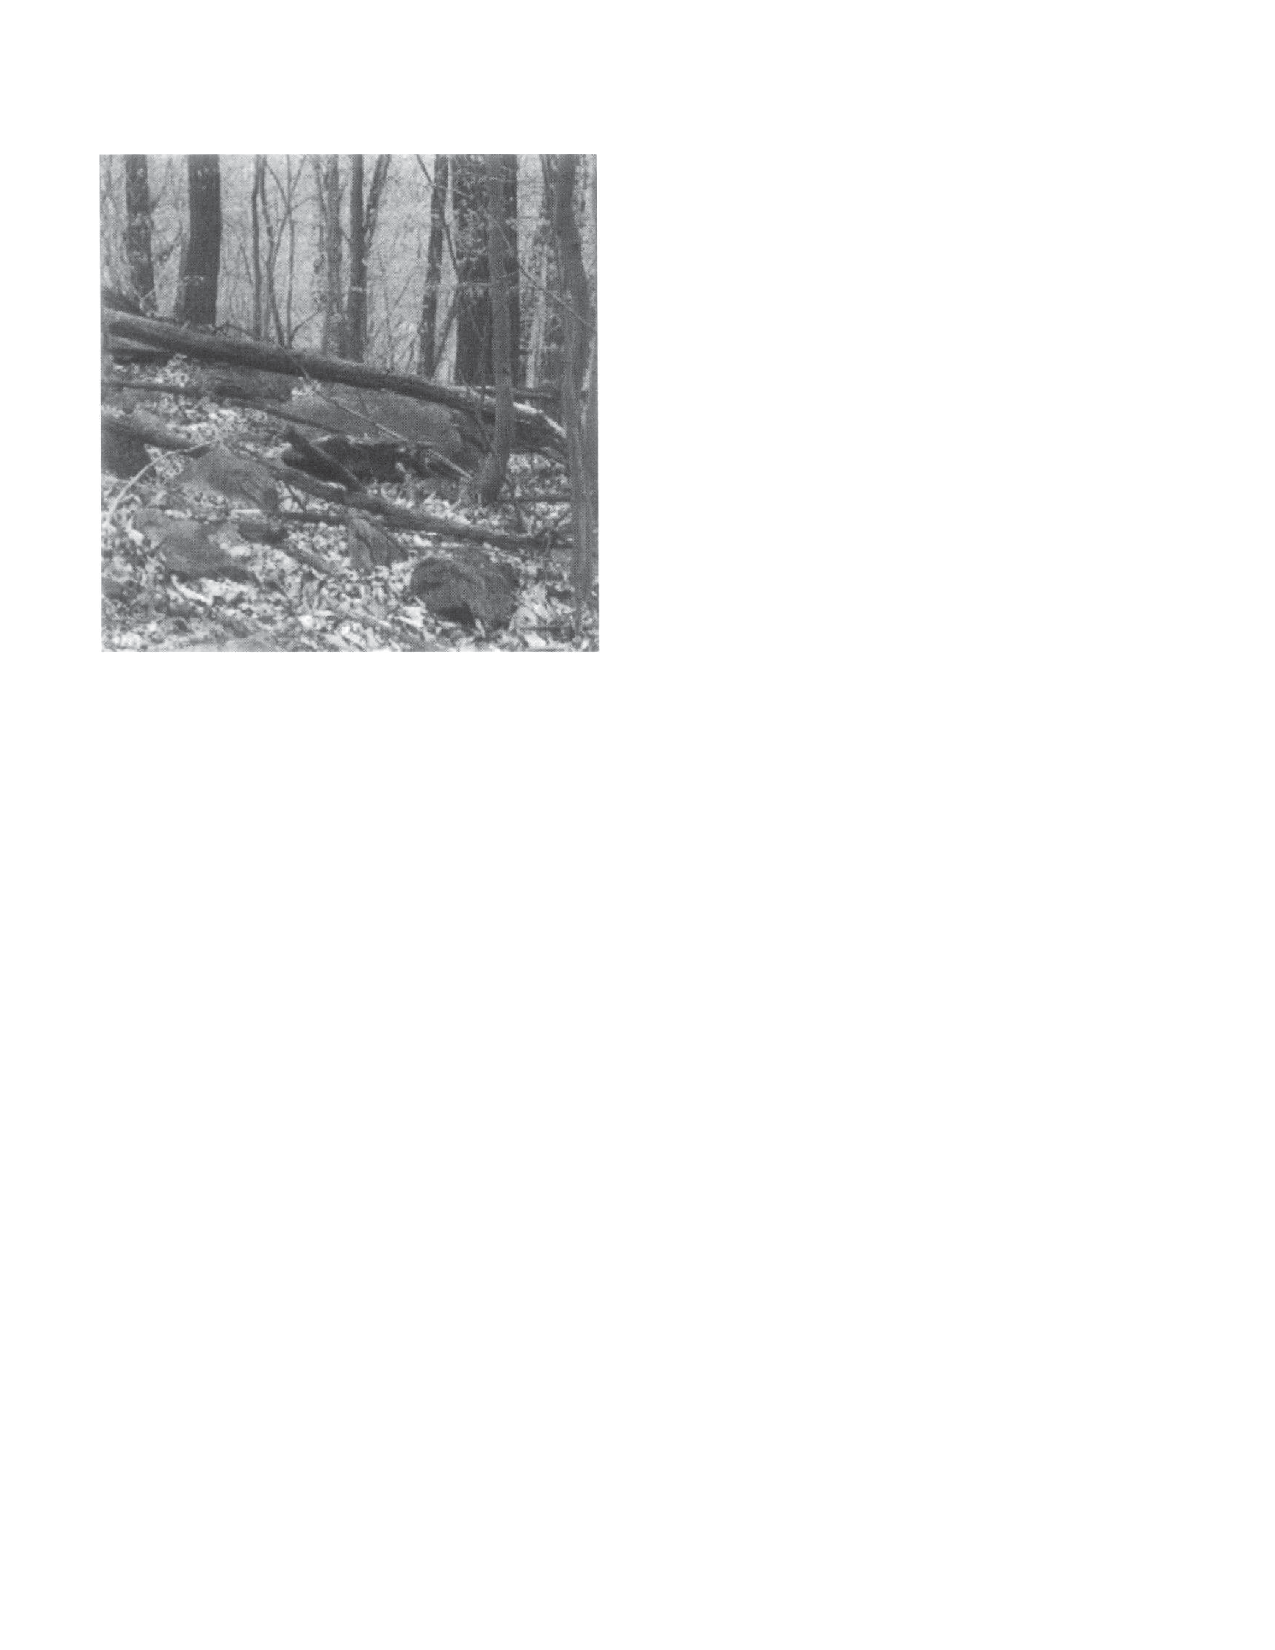
\includegraphics[scale=0.5]{figs/ruderman_bialek_img.pdf}
\hspace*{5 mm}
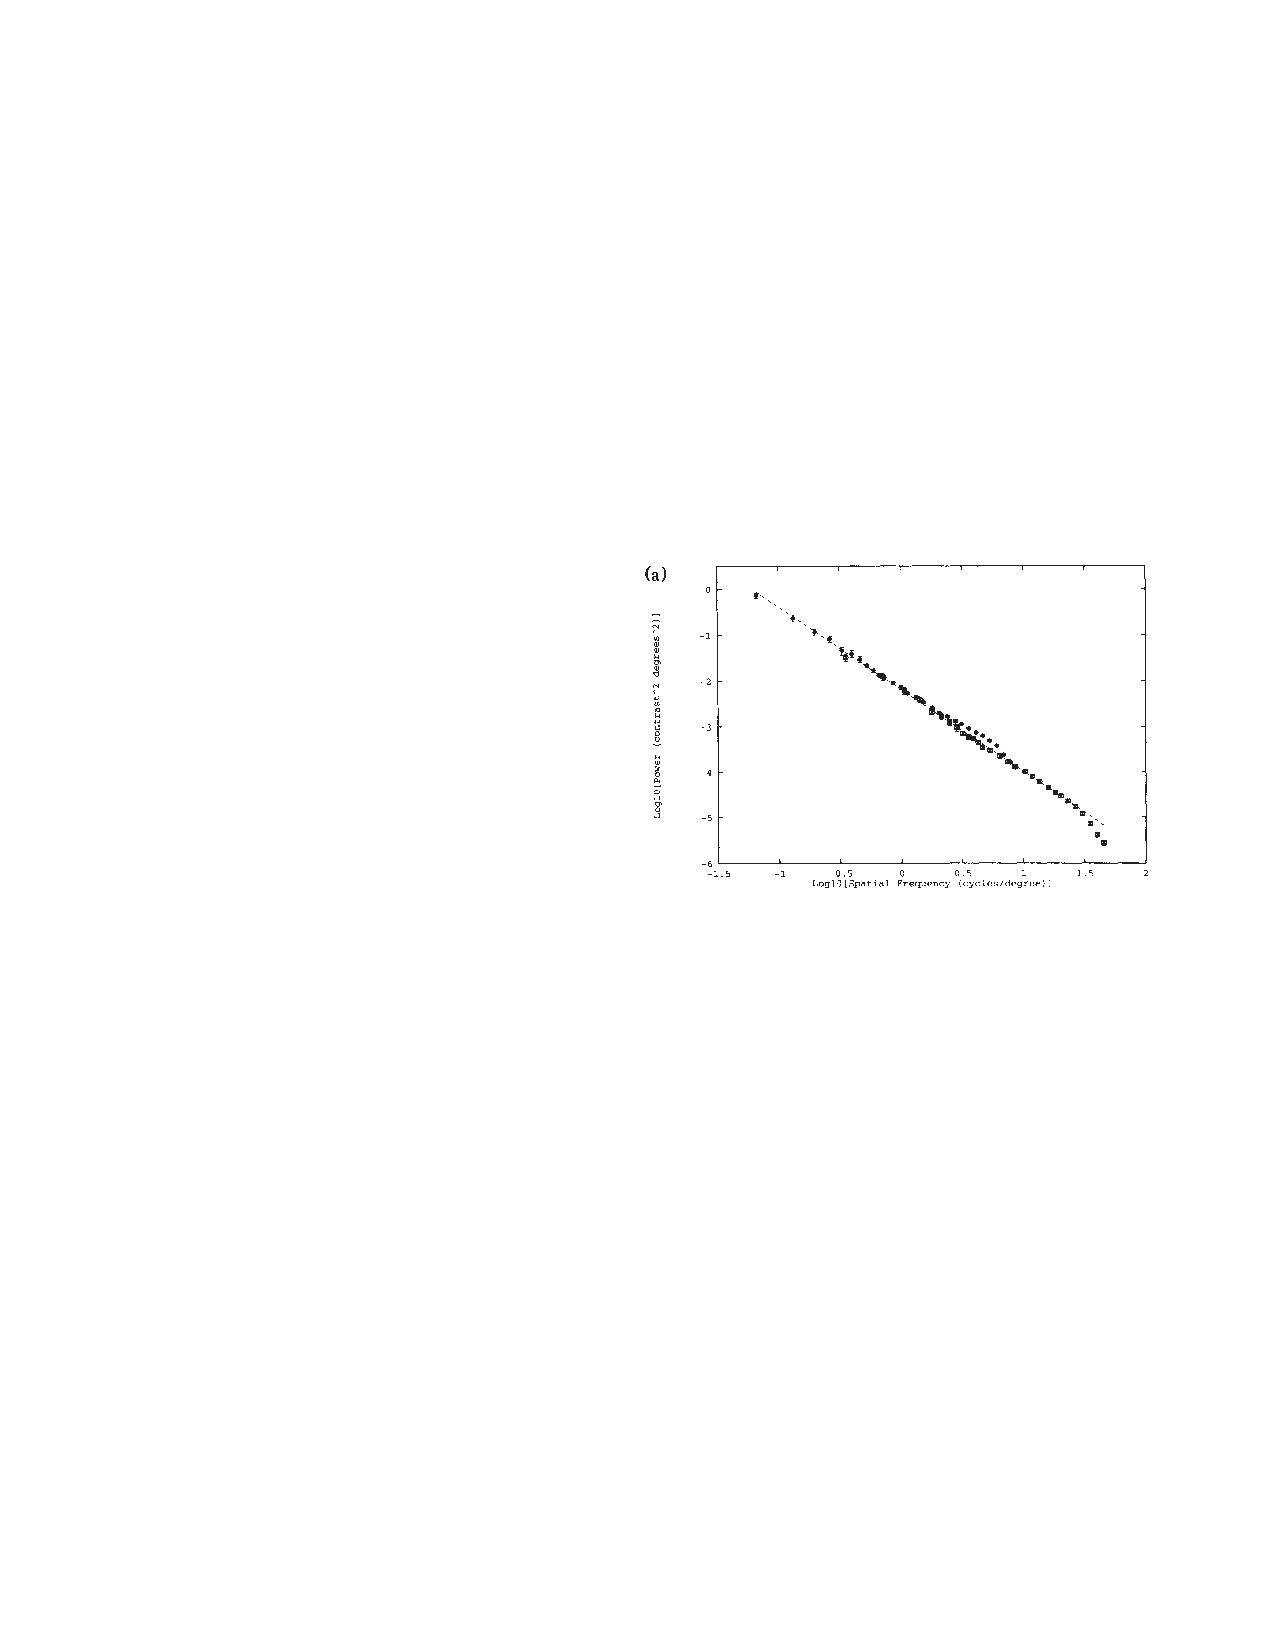
\includegraphics[scale=0.75]{figs/ruderman_bialek_plot.pdf}
\end{center}
}

\frame[t] {
\frametitle{Pitman Yor Process (PYP) : Definition \cite{Pitman1997a}}
 A Pitman-Yor process $\PY(c,d,H)$ is a distribution over distributions with three parameters:
\begin{itemize}
\item A discount $ 0 \le d < 1 $ that controls power-law behavior
\begin{itemize}
\item $d=0$ is DP
\end{itemize}
\item A concentration $c > -d$ like that of the DP
\item A base distribution $H$ also like that of the DP
\end{itemize}
A draw $G \sim PY(c,d,H)$ is also atomic

\[G = \sum_{k=1}^{\infty} \pi_k \delta_{\phi_k}\].  
}

\frame[t]{
\frametitle{PYP: Stick-Breaking Construction}
The procedure for generating a draw from a PYP is to draw $\pi_k$ from a generalized stick-breaking procedure and $\phi_k$ as usual:
\[
\begin{array}{rcll}
\beta_k  & \sim & \Bet(1-d, c+kd) & \forall \, k = 1 \ldots \infty \\
&&& \\
\pi_k & = &  \beta_k \prod_{i=1}^{k-1}(1- \beta_i) & \forall \, k = 1 \ldots \infty \\
&&& \\
\phi_k  & \sim &  H & \forall \, k = 1 \ldots \infty
\end{array}
\]

The expected length of a stick $\mathbb{E}[\pi_k]$ falls off as a power law for large $k$ when $d \ne 0$.  When $d = 0$ the stick lengths fall off exponentially, and the PYP reduces to a Dirichlet process.
%The expected length of a stick is $\mathbb{E}[\pi_k] = \mathbb{E}[\beta_k]\prod_{i=1}^{k-1}(1 - \mathbb{E}[\beta_i]) = \frac{1-d}{1+c+(k-1)d}\prod_{i=1}^{k-1}\frac{c+id}{1+c+(i-1)d} = d(1-d)\frac{\Gamma(\frac{c}{d} + (k-1))}{\Gamma(\frac{c}{d})}\frac{\Gamma(\frac{1+c}{d})}{\Gamma(\frac{1+c}{d} + k)}$
}

\frame[t] {
\frametitle{PYP: Power Law}
\begin{figure}[t]
\begin{center}
%\includegraphics[trim = 4cm 8cm 4cm 8cm, clip, width=5cm]{fig/shared_clustering.pdf}
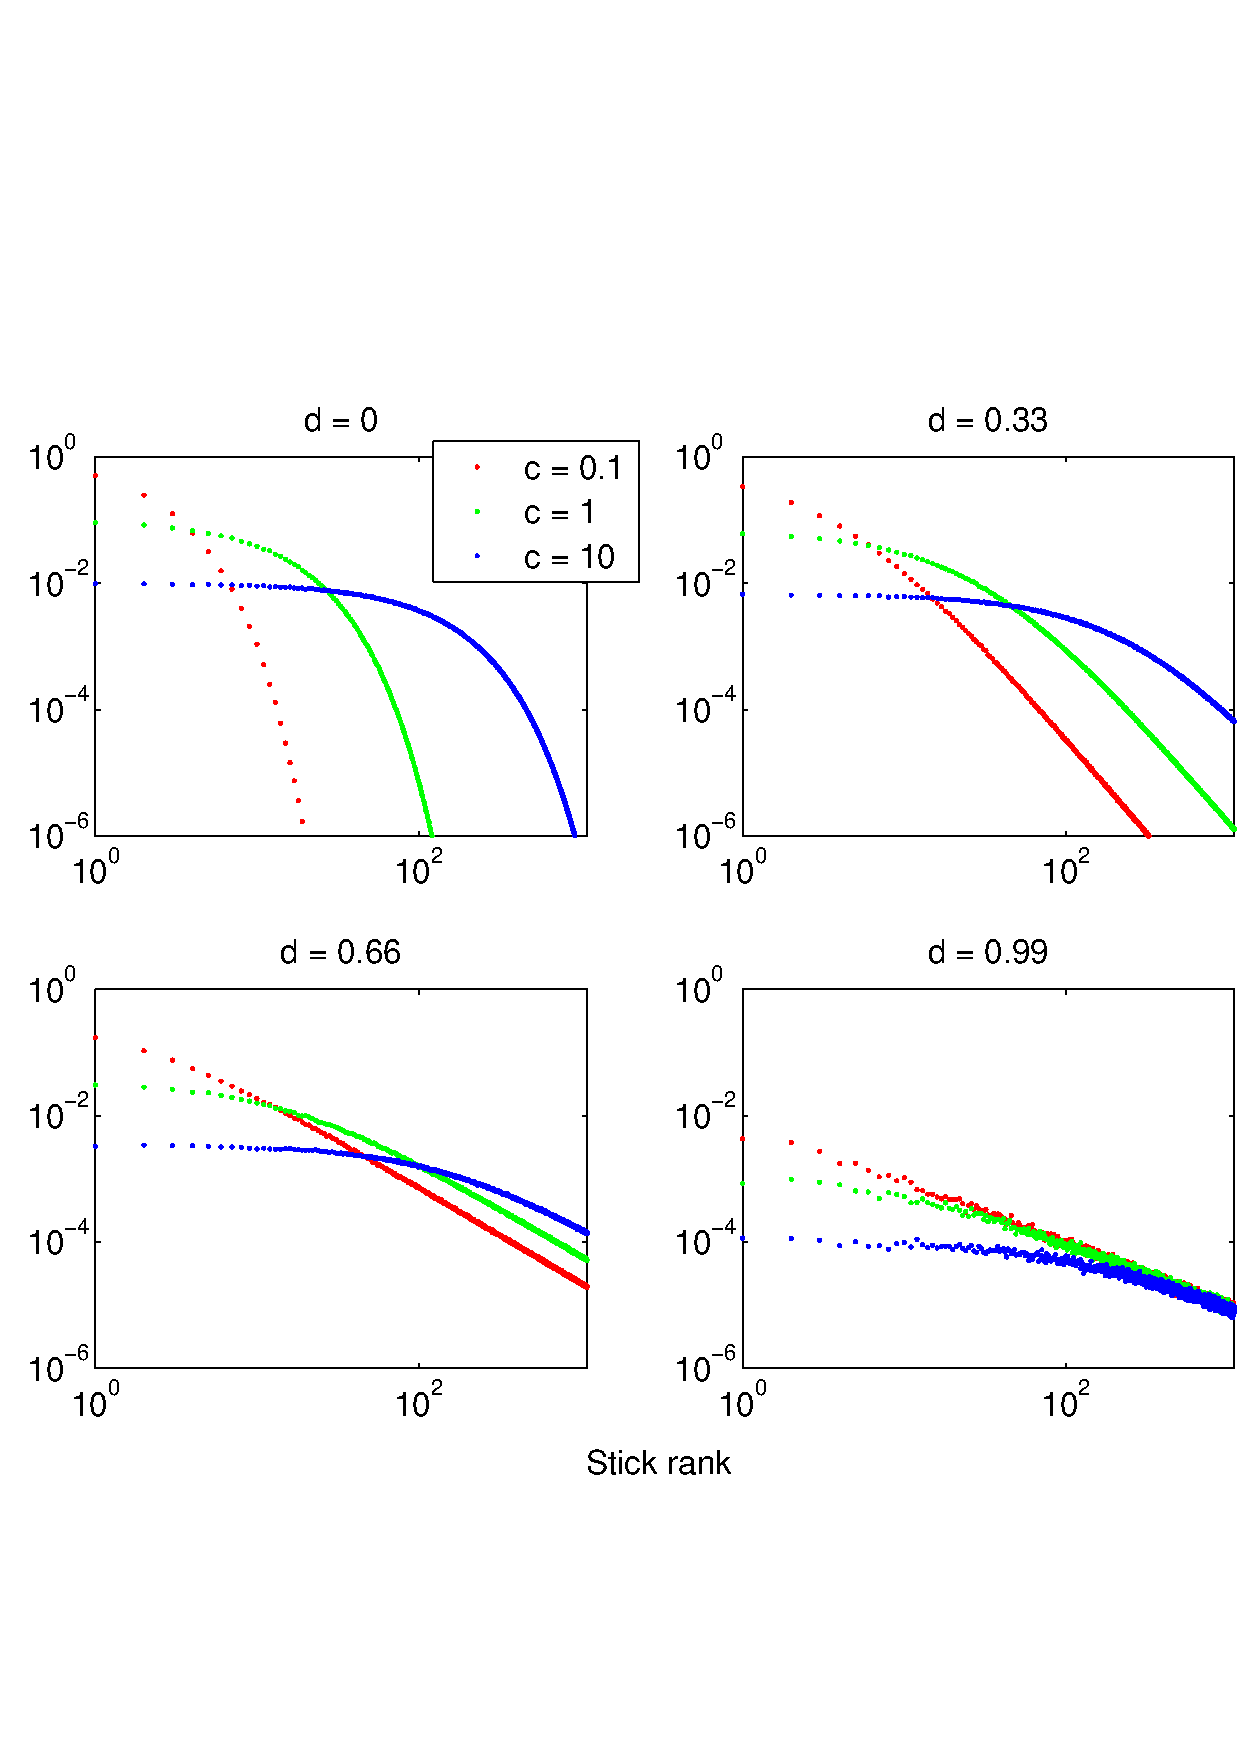
\includegraphics[width=8cm]{jtfig/pypl.pdf}
%\caption{Shared clustering}
\label{default}
\end{center}
\end{figure}
}

\frame[t] {
\frametitle{PYP: Polya Urn Representation}
As in the DP, the PYP posterior predictive distribution can be expressed with $G$ marginalized out.  
\begin{eqnarray*}
p(x_{n+1} | x_{1}, \ldots, x_n) & = & \Ave\left[\frac{m_k - d}{c+n}\delta(\phi_k-\cdot) + \frac{c + Kd}{c + n}H(\cdot)\right]
\end{eqnarray*}

This again forms the basis for similar SMC and MCMC inference algorithms.
\bigskip

Note: As in the case of the DP, due to the discrete nature of distributions $G \sim \PY(c,d,H)$, draws from $G$ tend to take the same value or ``cluster.''  
}

\frame[t] {
\frametitle{Hierarchical Pitman-Yor Process \cite{Teh2006a}}
A hierarchical Pitman-Yor process is the ``obvious'' two-parameter extension of the hierarchical Dirichlet process \cite{Teh2006b,Goldwater2006}.\\
\bigskip

Example:
%\begin{columns}[t]
%\begin{column}{.75\textwidth}
\begin{eqnarray*}
	\G_{[]} | \U_{\Sigma}, d_0 &\sim& \PY(d_0, 0, \U_{\Sigma }) \\
	\G_{\bf{u}} | \G_{\sigma(\bf{u})}, d_{|\bf{u}|} &\sim& \PY(d_{|\bf{u}|}, 0, \G_{\sigma(\bf{u})}) \hspace{.35cm} \forall {\bf u} \in \Sigma^+\\
	x_n | x_{n-1},  \ldots, x_1 = \bf{u} &\sim& \G_{\bf{u}}
\end{eqnarray*}
%\end{column}
%\begin{column}{.25\textwidth}
%\includegraphics[trim = 4cm 8cm 4cm 8cm, clip, width=5cm]{../../2010_icml/fig/sm_graphical_model.pdf}
%\todo{insert graphical model fig}
%\end{column}
%\end{columns}
%\bigskip
Estimation and inference follow that for the hierarchical Dirichlet process
}

\frame[t] {
\frametitle{Review}
\begin{block}{Summary}
\begin{itemize}
\item DP and PYP are flexible priors on distributions
\item Can think of either as glue for tying together related distributions in hierarchical models.
\item 
\end{itemize}
\end{block}
}
\section{Discrete Sequence Data}
\section{Compression}
\section{Thanks}

\begin{frame}{Data}
010101100100001010000000011101010010010101010010000101010101001010100101010
\end{frame}
	
\end{document}
